\documentclass[11pt,a4paper]{article}
%%%%%%%%%%%%%%%%%%%%%%%%%%%%%%%%%%%%%%%%%%%%%%%%%%%%%%%%
%                      PACKAGES                        %
%%%%%%%%%%%%%%%%%%%%%%%%%%%%%%%%%%%%%%%%%%%%%%%%%%%%%%%%

\usepackage[utf8]{inputenc}
\usepackage{graphicx} % Allows you to insert figures
\usepackage[export]{adjustbox}
\usepackage{booktabs}
\usepackage{amsmath} % Allows you to do equations
\usepackage{helvet}
\usepackage{hyperref}
\renewcommand{\familydefault}{\sfdefault}
\usepackage[a4paper, total={6.5in, 9.5in}]{geometry} % Formats the paper size, orientation, and margins
\linespread{1.1} % about 1.5 spacing in Word
\setlength{\parindent}{0pt} % no paragraph indents
\setlength{\parskip}{1em} % paragraphs separated by one line
\usepackage{listings}
\usepackage{enumitem}
\usepackage{xcolor}
\usepackage{hyperref}
\usepackage{pmboxdraw}
\usepackage{dirtree}

\hypersetup{
	colorlinks=true,
	urlcolor=cyan,
	linktoc=none,
}
\usepackage{fancyhdr}
\usepackage{float}

\pagestyle{fancy}
\fancyhead[L,C,R]{}
\fancyfoot[L]{Blix - AI Photo Editor}
\fancyfoot[C]{}
\fancyfoot[R]{\textbf{\thepage}}
\renewcommand{\headrulewidth}{0pt}
\renewcommand{\footrulewidth}{0.5pt}

\definecolor{codegreen}{rgb}{0,0.6,0}
\definecolor{codegray}{rgb}{0.5,0.5,0.5}
\definecolor{codepurple}{rgb}{0.58,0,0.82}
\definecolor{backcolour}{rgb}{0.95,0.95,0.92}

\usepackage{listings}

% Define TypeScript language style
\lstdefinelanguage{TypeScript}{
  keywords=[1]{class, constructor, let},
  keywordstyle=[1]\bfseries,
  keywords=[2]{string},
  keywordstyle=[2]\color{blue},
  sensitive=true,
  morestring=[b]',
  morestring=[b]"
}


\lstdefinestyle{mystyle}{
backgroundcolor=\color{backcolour},
commentstyle=\color{codegreen},
keywordstyle=\color{magenta},
numberstyle=\tiny\color{codegray},
stringstyle=\color{codepurple},
basicstyle=\ttfamily\footnotesize,
breakatwhitespace=false,
breaklines=true,
keepspaces=true,
numbers=left,
numbersep=5pt,
showspaces=false,
showstringspaces=false,
showtabs=false,
tabsize=2,
}

\lstset{style=mystyle}
\def\code#1{\texttt{#1}}

%%%%%%%%%%%%%%%%%%%%%%%%%%%%%%%%%%%%%%%%%%%%%%%%%%%%%%%%
%            TITLE PAGE & TABLE OF CONTENTS            %
%%%%%%%%%%%%%%%%%%%%%%%%%%%%%%%%%%%%%%%%%%%%%%%%%%%%%%%%

\begin{document}

\begin{titlepage}
	\centering
    % \includegraphics[width=0.5\textwidth]{your_logo.png}\par\vspace{1cm}
    {\scshape\LARGE User Manual Specification V1\par}
    \vspace{1.5cm}
    {\huge\bfseries Blix - AI Photo Editor\par}
    \vspace{2.5cm}
    \begin{figure}[h]
        \centering % center the image
        
\includegraphics[width=0.5\textwidth]{../pics/blix.png}
    \end{figure}
    \vspace{2.5cm}
    {\Large\itshape The Spanish Inquisition\par}

    \vfill
    {\large \today\par}
\end{titlepage}

\tableofcontents
\pagebreak

%%%%%%%%%%%%%%%%%%%%%%%%%%%%%%%%%%%%%%%%%%%%%%%%%%%%%%%%
%                MAIN DOCUMENT CONTENT                 %
%%%%%%%%%%%%%%%%%%%%%%%%%%%%%%%%%%%%%%%%%%%%%%%%%%%%%%%%

\addcontentsline{toc}{section}{Introduction}
\section*{Introduction}

Introducing Blix: An Advanced AI Photo Editor

Welcome to Blix, an innovative and sophisticated AI-powered photo editing application. Blix sets itself apart by providing users with a seamless editing experience through a powerful and 
intuitive interface, reminiscent of a digital blender. This user manual will guide you through the features and functionalities of Blix, enabling you to harness the full potential of 
this cutting-edge editing tool.

Blix caters to users of all levels, from amateur photographers to seasoned professionals, by streamlining the editing process and eliminating the need 
for extensive knowledge of complex editing software. By presenting a visual graph-based interface, akin to a blender, Blix enables effortless mixing and matching of diverse editing effects.

As a user, you gain access to a vast array of editing possibilities. Whether you wish to apply filters, fine-tune brightness and contrast, or add artistic effects such as vignettes or vintage tones, Blix provides an extensive selection of editing options. Each editing choice is represented as a node within the graph, allowing for seamless connectivity and the creation of custom editing flows tailored to your preferences.

What truly sets Blix apart is its integration of cutting-edge AI technology. Through Blix, you can engage with an AI assistant that enhances your editing journey. 
By sending prompts to the AI, you unlock a world of possibilities. The AI assistant can recommend specific edits, suggest optimal adjustments, or even manipulate the graph on your behalf, 
all based on your unique preferences and the desired outcome.

In summary, Blix is an advanced AI photo editor that empowers users to elevate their photography with ease and finesse. Its intuitive graph-based interface, extensive editing options, 
and integration with an AI assistant create a harmonious environment for realizing your creative vision. This user manual will serve as your comprehensive guide, enabling you 
to navigate the features of Blix and unlock the full potential of your photo editing capabilities.
\pagebreak


\addcontentsline{toc}{section}{Specifications}
\section*{Specifications}

\addcontentsline{toc}{subsection}{Hardware Requirements}
\subsection*{Hardware Requirements}
\begin{itemize}
  \item[\textbullet] \textbf{2 GB RAM}
  \item[\textbullet] \textbf{1.8Ghz }.

\end{itemize}

\addcontentsline{toc}{subsection}{System Requirements}
\subsection*{System Requirements}

Blix is compatible with the following operating systems:
\begin{itemize}
  \item[\textbullet] \textbf{Windows}
  \item[\textbullet] \textbf{Linux }.
  \item[\textbullet] \textbf{MacOS }.
\end{itemize}

 Internet connection is not required, however additional features are available when connected to the internet.

\addcontentsline{toc}{section}{Usage}
\section*{Usage}

\textbf{Useful bindings}
\begin{itemize}
  \item[\textbullet] Command palette : \textbf{Ctrl + P}
  \item[\textbullet] Delete Node : \textbf{Ctrl + del}
  \item[\textbullet] Add Node : \textbf{Ctrl + A}
\end{itemize}

\begin{figure}[H]
  \centering
  {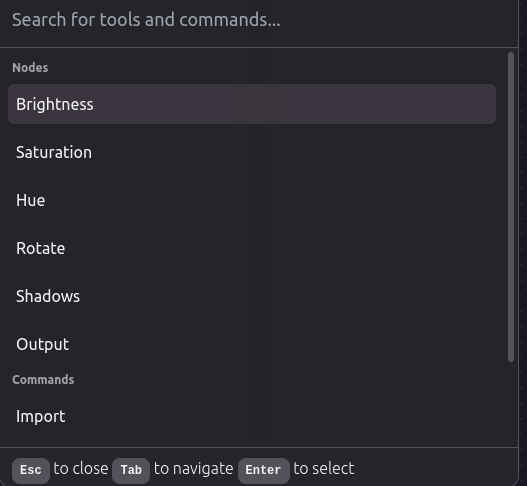
\includegraphics[width=0.5\textwidth]{../pics/palette.png}}
  \caption{Command Palette}
\end{figure}


\addcontentsline{toc}{subsection}{Projects}
\subsection*{Projects}

Projects form the basis of Blix. A project is a collection of images and their associated editing graphs. Projects are saved locally on your machine and can be accessed at any time. 
Alternatively these projects can be exported and shared with other users. When you open Blix, you will either see the projects you have previously created or a blank canvas to create new projects.

\textbf{Saving a project}
When you have the main app open, you can create a project as follows : 

\begin{itemize}
  \item[\textbullet] Click on the + icon in the top left corner of the screen.
  \item[\textbullet] Click on file in the top left and select save project, or choose the save file command in the command palette.
  \item[\textbullet] Select a directory and file name for the project. Save.
\end{itemize}

\textbf{Importing a project}
Projects will automatically be loaded when you open Blix. If you wish to import a project, you can do so as follows : 

\begin{itemize}
  \item[\textbullet] Select file in the top left corner of the screen.
  \item[\textbullet] Select import project, or choose the import file command in the command palette.
  \item[\textbullet] Select the project you wish to import.
\end{itemize}

\textbf{Deleting a project}
Projects can be permanently removed from your workspace as follows : 
\begin{itemize}
  \item[\textbullet] Select file in the top left corner of the screen.
  \item[\textbullet] Select delete project, or choose the delete file command in the command palette.
  \item[\textbullet] Select the project you wish to delete.
\end{itemize}

\addcontentsline{toc}{subsection}{Photo editing}
\subsection*{Photo editing}

\textbf{Importing a Photo}

Images can be added to the graph as input. This can be done using the input plugin : 
\begin{itemize}
  \item[\textbullet] Select the Image input node.
  \item[\textbullet] Place the node in the tile you wish to add the image to.
  \item[\textbullet] Use the interface provided to import the image to the node.
  \item[\textbullet] Connect the image to the graph.
\end{itemize}

\textbf{Adding nodes to a graph}

There are a wide array of nodes that can be added to the workspace area.
\begin{itemize}
  \item[\textbullet] Select the node from either the command palette or the nodes pane.
  \item[\textbullet] Place the node in the tile you wish to add the image to.
  \item[\textbullet] Connect the node to the graph.
\end{itemize}

\begin{figure}[H]
  \centering
  \href{https://www.youtube.com/watch?v=ak3Bto3phqk}
  {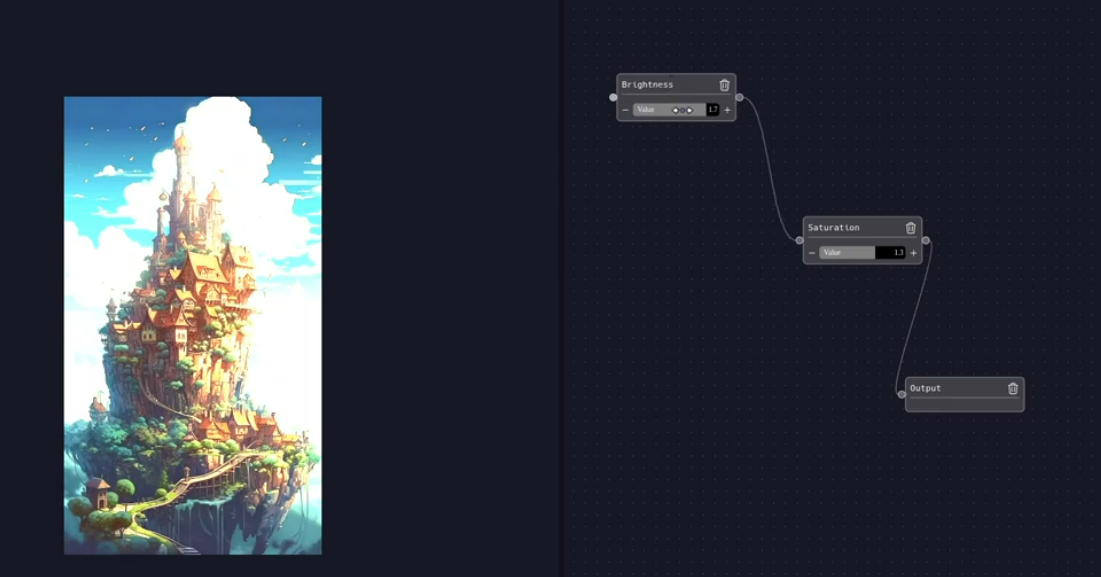
\includegraphics[width=0.5\textwidth]{../pics/nodes.png}}
\end{figure}


\textbf{Editing a Photo}

Images can be edited in the graph using the various editing nodes. These nodes can be connected to the image input node to apply the desired effect.
The nodes will perform manipulations on the image and output the result. This result can then be connected to other nodes to create a chain of effects.
It should be noted that this functionality does not only apply to images, but to any input given.

\textbf{Exporting a Photo}

Photos can be exported to a format of your choice. This can be done as follows :

\begin{itemize}
  \item[\textbullet] Select file in the top left corner of the screen or open the command palette.
  \item[\textbullet] Select export image.
  \item[\textbullet] The image of your currently active workspace will be exported to the directory of your choice.
\end{itemize}

\addcontentsline{toc}{subsection}{Layout Customization}
\subsection*{Layout Customization}

Blix prides itself on its intuitive and user-friendly interface. The layout of the application is highly customizable, enabling you to tailor the interface to your preferences.

\textbf{Changing the panels layout}

Blix allows a wide array of customizablity for the panels layout. You can customize the panel layout as follows :

\begin{itemize}
  \item[\textbullet] Panel borders can be changed by dragging the borders of the panels.
  \item[\textbullet] Panels can be moved by dragging the panel header.
  \item[\textbullet] Panels can be closed by dragging the blip upwards.
  \item[\textbullet] Panels can be duplicated by dragging the blip downwards or sideways.
\end{itemize}


\addcontentsline{toc}{subsection}{Plugins}
\subsection*{Plugins}

One of the core features of Blix is its plugin system. This system allows users to create their own plugins and add them to the application. This enables users to create their own custom nodes and 
add them to the graph. This section will serve as a guide to creating your own plugins.

\textbf{Using plugins}

Blix ensures that every node in the graph is a plugin. This means that all node functionality is extremely extensible and add them to the graph. Key features include : 

\begin{itemize}
  \item[\textbullet] Plugin files are stored in the blix-plugins folder.
  \item[\textbullet] Users can create their own plugins and share them with other users.
  \item[\textbullet] Every property of the node is defined in the plugin file.
\end{itemize}

\textbf{Creating plugins}

Blix allows users to create and customize their own plugins with an elegant and intuitive interface. Users can define nodes, commands and tiles.

\begin{itemize}
  \item[\textbullet] Nodes are constructed using the dedicated nodeBuilders provided in our docs.
  \item[\textbullet] Commands are more loosely created by users, however well defined commands are provided in our system.
  \item[\textbullet] Tiles are created using the dedicated tileBuilders provided in our docs.
\end{itemize}


\end{document}